\documentclass[oneside]{book}

\usepackage{amsmath, amsthm, amssymb, amsfonts}
\usepackage{thmtools}
\usepackage{graphicx}
\usepackage{setspace}
\usepackage{geometry}
\usepackage{float}
\usepackage{hyperref}
\usepackage[utf8]{inputenc}
\usepackage[english]{babel}
\usepackage{framed}
\usepackage{tikz}
\usetikzlibrary{shapes.geometric}\usepackage[dvipsnames]{xcolor}
\usepackage{environ}
\usepackage{tcolorbox}
\newcommand{\bA}{\mathbf{A}}
\newcommand{\bB}{\mathbf{B}}
\newcommand{\bC}{\mathbf{C}}
\newcommand{\bD}{\mathbf{D}}
\newcommand{\bE}{\mathbf{E}}
\newcommand{\bF}{\mathbf{F}}
\newcommand{\bG}{\mathbf{G}}
\newcommand{\bH}{\mathbf{H}}
\newcommand{\bI}{\mathbf{I}}
\newcommand{\bJ}{\mathbf{J}}
\newcommand{\bK}{\mathbf{K}}
\newcommand{\bL}{\mathbf{L}}
\newcommand{\bM}{\mathbf{M}}
\newcommand{\bN}{\mathbf{N}}
\newcommand{\bO}{\mathbf{O}}
\newcommand{\bP}{\mathbf{P}}
\newcommand{\bQ}{\mathbf{Q}}
\newcommand{\bR}{\mathbf{R}}
\newcommand{\bS}{\mathbf{S}}
\newcommand{\bT}{\mathbf{T}}
\newcommand{\bU}{\mathbf{U}}
\newcommand{\bV}{\mathbf{V}}
\newcommand{\bW}{\mathbf{W}}
\newcommand{\bX}{\mathbf{X}}
\newcommand{\bY}{\mathbf{Y}}
\newcommand{\bZ}{\mathbf{Z}}

%% blackboard bold math capitals
\newcommand{\bbA}{\mathbb{A}}
\newcommand{\bbB}{\mathbb{B}}
\newcommand{\bbC}{\mathbb{C}}
\newcommand{\bbD}{\mathbb{D}}
\newcommand{\bbE}{\mathbb{E}}
\newcommand{\bbF}{\mathbb{F}}
\newcommand{\bbG}{\mathbb{G}}
\newcommand{\bbH}{\mathbb{H}}
\newcommand{\bbI}{\mathbb{I}}
\newcommand{\bbJ}{\mathbb{J}}
\newcommand{\bbK}{\mathbb{K}}
\newcommand{\bbL}{\mathbb{L}}
\newcommand{\bbM}{\mathbb{M}}
\newcommand{\bbN}{\mathbb{N}}
\newcommand{\bbO}{\mathbb{O}}
\newcommand{\bbP}{\mathbb{P}}
\newcommand{\bbQ}{\mathbb{Q}}
\newcommand{\bbR}{\mathbb{R}}
\newcommand{\bbS}{\mathbb{S}}
\newcommand{\bbT}{\mathbb{T}}
\newcommand{\bbU}{\mathbb{U}}
\newcommand{\bbV}{\mathbb{V}}
\newcommand{\bbW}{\mathbb{W}}
\newcommand{\bbX}{\mathbb{X}}
\newcommand{\bbY}{\mathbb{Y}}
\newcommand{\bbZ}{\mathbb{Z}}

%% script math capitals
\newcommand{\sA}{\mathscr{A}}
\newcommand{\sB}{\mathscr{B}}
\newcommand{\sC}{\mathscr{C}}
\newcommand{\sD}{\mathscr{D}}
\newcommand{\sE}{\mathscr{E}}
\newcommand{\sF}{\mathscr{F}}
\newcommand{\sG}{\mathscr{G}}
\newcommand{\sH}{\mathscr{H}}
\newcommand{\sI}{\mathscr{I}}
\newcommand{\sJ}{\mathscr{J}}
\newcommand{\sK}{\mathscr{K}}
\newcommand{\sL}{\mathscr{L}}
\newcommand{\sM}{\mathscr{M}}
\newcommand{\sN}{\mathscr{N}}
\newcommand{\sO}{\mathscr{O}}
\newcommand{\sP}{\mathscr{P}}
\newcommand{\sQ}{\mathscr{Q}}
\newcommand{\sR}{\mathscr{R}}
\newcommand{\sS}{\mathscr{S}}
\newcommand{\sT}{\mathscr{T}}
\newcommand{\sU}{\mathscr{U}}
\newcommand{\sV}{\mathscr{V}}
\newcommand{\sW}{\mathscr{W}}
\newcommand{\sX}{\mathscr{X}}
\newcommand{\sY}{\mathscr{Y}}
\newcommand{\sZ}{\mathscr{Z}}


\renewcommand{\emptyset}{\O}

\newcommand{\abs}[1]{\lvert #1 \rvert}
\newcommand{\norm}[1]{\lVert #1 \rVert}
\newcommand{\sm}{\setminus}


\newcommand{\sarr}{\rightarrow}
\newcommand{\arr}{\longrightarrow}

\newcommand{\hide}[1]{{\color{red} #1}} % for instructor version
%\newcommand{\hide}[1]{} % for student version
\newcommand{\com}[1]{{\color{blue} #1}} % for instructor version
%\newcommand{\com}[1]{} % for student version
\newcommand{\meta}[1]{{\color{green} #1}} % for making notes about the script that are not intended to end up in the script
%\newcommand{\meta}[1]{} % for removing meta comments in the script

\DeclareMathOperator{\ext}{ext}
\DeclareMathOperator{\ho}{hole}
\tcbuselibrary{theorems,skins,breakable}

\setstretch{1.2}
\geometry{
    textheight=9in,
    textwidth=5.5in,
    top=1in,
    headheight=12pt,
    headsep=25pt,
    footskip=30pt
}

% Variables
\def\notetitle{Apprentice Lectures}
\def\noteauthor{
    \textbf{Daniil Rudenko} \\ 
    {\LaTeX} by Agustin Esteva}
\def\notedate{\today}

% The theorem system and user-defined commands
\input{theorems.tex}
\input{commands.tex}

% ------------------------------------------------------------------------------

\begin{document}
\title{\textbf{
    \LARGE{\notetitle} \vspace*{10\baselineskip}}
    }
\author{\noteauthor}
\date{\notedate}

\maketitle
\newpage

\tableofcontents
\newpage

% ------------------------------------------------------------------------------

\chapter{Lecture 1- Combinatorics and Isometries}
\section{Combinatorics}
\ex{How many subsets of $A = \{1,2,\dots, n\}$? $2^n.$}
\pf{(By Induction)\newline
\begin{enumerate}
    \item If $A = \{1\}$ then there exists $\emptyset$ and $\{1\}$ as subsets of $A.$ Thus there exist $2^1 =2$ subsets.
    \item If $A = \{1,2, \dots, n-1\},$ then assume that there exist $2^{n-1}$ subsets of $A.$
    \item If $n,$ then let $Y = \{1,2,\dots, n-1\}$ and $X = \{1,2\dots, n\}.$ Evidently, there exists an isomorphism between $Y$ and $A,$ and thus there are $2^{n-1}$ subsets in $Y.$ Let $f: X\to X\setminus\{n\}.$ Now, $X$ is in bijective correspondence with $A,$ and thus there are $2^{n-1}$ subsets in $X.$ Therefore, there are $2^{n-1}+2^{n-1} = 2^n$
\end{enumerate}}
\pf{(With Linear Algebra)\newline
It will suffice to show that $[2^n]$ (the power set of any set with cardinality $n,$ is isomorphic to $\bbF_2^n.$)\newline
First, to show that $[2^n]$ is a valid vector field of $\bbF_2$ with multiplication and addition defined as follows: If $X,Y \in [2^n],$ then:
\[X + Y = X \Delta Y = (X\sm Y)\cup (Y \sm X) \qquad 1 \cdot X = X \qquad 0\cdot X = \emptyset\]
\begin{enumerate}
    \item Commutativity, to prove that $X + Y = Y + X,$ it will suffice to show that the symmetric difference is commutative, which it is. 
    \item $\Delta$ is associative.
    \item There exists a $\emptyset$ in $[2^n]$ such that $X + \emptyset = X \Delta \emptyset = X.$
    \item The additive inverse is $-X = X$. To prove this, note that $-X + X = X \Delta X = \emptyset.$
    \item $1$ is multiplicative identity by definition.
    \item All the rest of the axioms are similarly proved.
\end{enumerate}
}
\defn{Binomial Coefficients}{The number of subsets of size $k$ in the set $\{1,2,\dots, n\},$ usually denoted by $\binom{n}{k}$}
\rmkb{From the previous example, it is evident that \[\sum_{i =1}^n\binom{n}{i} = 2^n\]}

\thm{Binomial Coefficient Identity}{\[\binom{n}{k} = \binom{n}{n-k}\]}
\pf{Let $X$ be a subset of $A = \{1,2,\dots, n\}$ of size $k.$  Let $f: X \to A\sm X$ be a function and $g: Y \to A\sm Y$ be a function, where $Y$ is a set in the domain of $f.$ It will suffice to show that $g \circ f$ is a bijection. Let $gf(X_1) = gf(X_2).$ Therefore, because $A\sm(A\sm X_1) = X_1$ and $A\sm(A\sm X_2) = X_2,$ then $X_1 = X_2,$ and so $g\circ f$ is injective. Assume that there exists some $X$ such that $X \neq A\sm(A\sm X).$ However, this is impossible.}

\rmkb{This result (and the next) lead to an interesting way to represent binomial coefficients:}
\begin{figure}[h!]
    \centering
    \includegraphics[width=0.5\linewidth]{REU-2024//Images/Pascal's Triangle.png}
    \caption{Pascal's Triangle for Binom. Coefficients}
    \label{fig:enter-label}
\end{figure}
\thm{Morgan's Identity}{$\binom{n}{k} = \binom{n-1}{k} + \binom{n-1}{k-1}$}

\pf{Let $X$ be the subsets of size $k$ containing the element $n$ and let $Y$ be the subsets of size $k$ not containing $n.$ Like in Example 1, $Y$ is in bijective correspondence with the subsets of $\{1,2,\dots, n-1\}$ of size $k.$ Moreover, $X$ is also in bijective correspondence with subsets of $\{1,2,\dots, n-1\}$ of size $k-1$ (since you must take away an element, the sizes of the subsets decreases).}

\section{Isometries}

\defn{Isometry}{A map $f: \bbR^2 \to \bbR^2$ is an \textit{isometry} if:
\begin{enumerate}
    \item It is bijective.
    \item Distance is preserved, i.e, for all $x,y \in \bbR^2,$ $|xy| = |f(x)f(y)|$
\end{enumerate}}
\newcommand{\Isom}{\text{Isom}}
\ex{
\begin{enumerate}
    \item The identity map is an example of an isometry.
    \item We call the map $\bbS_O: \bbR^2 \to \bbR^2$ a symmetric difference, as it reflects points across some specified point, $O.$ Thus, $\bbS_O(X) = Y,$ where $O$ is the middle of the segment $[XY].$ Note that $\bbS_O$ preserves distances as given any $X_1,X_2 \in \bbR^2,$ the triangles $\triangle X_1OX_2 \sim Y_1OY_2,$ and thus $|X_1X_2| = |Y_1Y_2|.$
    \rmkb{$\bbS_O \circ \bbS_O = \text{Id}$}
    \item A translation, or a parallel transport, is a function, $T_\textbf{v}: \bbR^2 \to \bbR^2$ such that given some vector $\textbf{v}$ and some $X \in \bbR^2,$ then $T_\textbf{v}(X) = Y$ such that $\overrightarrow{XY} = \textbf{v}.$ 
    \rmkb{A vector, \textbf{v}, is defined as follows:
    \begin{enumerate}
        \item \[\textbf{v} = (\text{segment} + \text{orientation})\mod \text{\sim},\] where, given any $ABCD \in \bbR^2,$ $\sim$ is defined by:
        \begin{enumerate}
            \item $|AB| || |CD|$ (equivalent vectors are parallel).
            \item $|AB| = |CD|$ (equivalent vectors have the same magnitude).
            \item $B,D$ are on the same side of $AC$ (equivalent vectors have the same orientation).
        \end{enumerate}
    \end{enumerate}}
    \item A rotation around some point, $O \in \bbR^2,$ by $\varphi$ degrees, is a map $R_O^\varphi(X) = Y$ such that $|OX| = |XY|$ and there is a counterclockwise rotation from $\overline{OX}$ to $\overline{XY}$ by $\varphi$ degrees
\end{enumerate}}

\fact{If $f,g \in \Isom(\bbR^2),$ then $f\circ g \in \Isom(\bbR^2).$}
\pf{
\begin{enumerate}
    \item The compositions of bijections is a bijection, and thus $f\circ g$ is a bijection.
    \item Given any $X_1X_2 \in \bbR^2,$ since $g$ and $f$ preserves distances since it's an isometry, then \[|(f\circ g)(X_1)(f\circ g)(X_2)| = |fg(X_1)fg(X_2)| = |g(X_1)g(X_2)| = |X_1X_2|.\]
\end{enumerate}
}

\newpage

\chapter{Lecture 2- The Binomial Theorem/Formula and Groups}
\section{The Binomial Formula}
\thm{The Binomial Theorem}{\[(a+b)^n = \sum_{k=0}^n \binom{n}{k}a^{n-k}b^k\]}
Before this proof, it will be useful to understand how this works for $(a+b)^3.$ To do this, let's decompose the expression:
\[(a+b)^3 = (a+b) \cdot (a+b)\cdot (a+b)\] This, of course, yields \[aaa + aab + aba + baa + abb + bba + bab + bbb\] and this is equal to \[a^3 + 3a^2b + 3ab^2 + b^3.\] Note that if we count the brackets in the first expression as say, $1,2,3,$ thus we have the set $\{1,2,3\},$ where each element encodes a pair of brackets, then for the second expression we could denote this as all the possible subsets of $\{1,2,3\},$ where if the element appears, an $a$ is placed, and if not, then a $b$ is placed. Thus, the subset $\{1,3\}$ corresponds to $aba$ and the emptyset corresponds to $bbb.$
Therefore, \[a^3 + 3a^2b + 3ab^2 + b^3 = \sum_{X\subseteq \{1,2,3\}} \prod_{1\leq i \leq 3}(\text{an $a$ if $i \in X$ and $b$ if $i \notin X.$}) = \sum_{X \in \{1,2,3\}} a^{|X|}b^{3-|X|}\]
\pf{As the example above hows, \[(a+b)^n = (a+b)\cdot (a+b)\cdots (a+b) \{\text{n-times}\} = \sum_{X\subseteq \text{set of $\{1,2,3,\dots, n\}$}} a^{|X|}b^{n-|X|} = \sum_{k=0}^n\binom{n}{k}a^kb^{n-k}\]}
\rmkb{One could pretty easily do binomial expansion using Pascal's Triangle, the coefficients are just the numbers in the triangle.}

\cor{\[2^n = \binom{n}{0}+ \binom{n}{1} + \binom{n}{2} + \dots + \binom{n}{n}\]}
\pf{\[2^n = (1+1)^n = \binom{n}{0}+ \binom{n}{1} + \binom{n}{2} + \dots + \binom{n}{n}\]}

\thm{The Binomial Coefficient Formula}{\[\binom{n}{k} = \frac{n!}{k!(n-k)!}\]}
Before this proof, consider $5=5.$ This is a trivial statement, but it can mean a lot of things. Do $5$ crocodiles equal $5$ ducks? That's ridiculous!
\textbf{$5=5$ but not in a unique way.}\newline In fact, \[\text{permuting a set of $n$ obects $=$ $\#$ bijections from $\{1,2,\dots, n\}$ to itself $=$ $n!$ $=$ $\bbS_n$}\]
\pf{Count the number of permutations in two different ways. The first is by permuting everything using a factorial. The second is to choose $k$ elements out of the $n,$ then seeing how many permutations can occur within those $k$ elements, then seeing how many can occur in the $n-k$ elements. Thus $n! = \binom{n}{k}k!(n-k)!,$ and we are done, as rearranging this yields the thesis.}
\cor{A set of size $n$ has $2^{n-1}$ even subsets}
\pf{
\begin{enumerate}
    \item If $n$ is even, then $(-1+1)^n = \binom{n}{0} - \binom{n}{1} + \binom{n}{2} + \dots + \binom{n}{n} = 0,$ and so by moving all the negative terms to the right, \[\sum_{k=2i}\binom{n}{k} = \sum_{k= 2i+1}\binom{n}{k}\] and thus because there are the same number of even and odd subsets, we get $2^{n-1}$ subsets.
    \item If $n$ is odd, then let $f: 2^A \to 2^A$ such that if $X \in 2^A,$ then $f(X) = A\sm X,$ and thus because this map is bijective, then there are the same number of $X$ as $A\sm (X),$ and since those have different parity, then there are the same number of even and odd sets.
\end{enumerate}
\rmkb{One could also try this using Linear Algebra, as consider the subspace $W \subseteq 2^A = V$ of all the even subsets.Note that because addition was defined on this vector space as $\Delta,$ and $\Delta$ is mantains parity of evens, then $W$ is a valid subspace. Consider that $|V| = 2^n = 2^{\dim(V)}.$ Thus, $|W| = 2^{\dim(W)}.$ Consider that $\beta = \{\{1,2\}, \{2,3\}, \dots, \{n-1,n\}\}$ is a valid basis of $W,$ and thus we are done.}
}

\section{Introduction to Groups}
\ex{Consider the following two statements:
\[T_\textbf{v}\circ T_\textbf{w} = T_{\textbf{v} + \textbf{w}}\qquad S_{O_2} \circ S_{O_2} = T_{2\overrightarrow{O_1O_2}}\] These proves should be clear geometrically.
}
\defn{Group}{A \textit{group}, $G$, is a set with an operation $G\times G \to G$ such that $(g_1,g_2) \to g_1 * g_2$ such that: 
\begin{enumerate}
    \item For all $g_1,g_2,g_3 \in G,$ $(g_1 * g_2) * g_3 = g_1 * (g_2 * g_3).$
    \item There exists a unit, $e\in G,$ suchat that $g * e = e*g = g.$
    \item For all $g\in G,$ there exists a $g',$ usually denoted as $g^{-1},$ or then inverse of $g,$ such that $g * g^{-1} = e.$
\end{enumerate}}


\begin{table}[h!]
    \centering
    \begin{tabular}{ccc}
         & Object & Operation ($*$)\\
       1  & $\bbZ$ & $+$\\
        2 & $\bbR$ & $+$ \\
         3&  $\bbR\sm \{0\}$& $\times$\\
         4&  $\Isom(\bbR^2)$&$\circ$ \\
         5& $\bbS_n$ & $\circ$\\
         6& $GL_n(F),$ or Invertible matrices of size $n\times n$ & $\times $\\
    \end{tabular}
    \caption{Common Groups}
    \label{Groups}
\end{table}

\chapter{Lecture 3- Groups and Catalan Numbers}
\section{Groups}
\defn{Abelian Group}{An \textit{Abelian Group} is a group in which, $*,$ the operation of the group, is commutative.}

\ex{For \Isom($\bbR^2$), it is generally not the case that $f\circ g = g\circ f,$ as is evidenced by the first example in 2.2}

\ex{More examples of groups:
\begin{enumerate}
    \item $G = \{e\}$
    \item $G = \{e,x\}$
    and thus $x$ must be its own inverse. Some examples include $G = \{-1,1\}, \times$ and $G  = \{0,1\}\subset \bbF_2, +$
    \item $G = \{e,x,y\}$
\end{enumerate}
}
Table for ex 2:
    \begin{table}[h!]
        \centering
        \begin{tabular}{ccc}
            * & $e$ & $x$\\
            $e$ & $e$ & $x$\\
            $x$ & $x$ & $e$ \\
        \end{tabular}
    \end{table}
\newline Table for ex 3:
    \begin{table}[h!]
        \centering
        \begin{tabular}{cccc}
            *  & $e$ & $x$ & $y$\\
            $e$& $e$ & $x$&  $y$   \\
            $x$& $x$ & $y$&  $e$\\
            $y$& $y$ & $e$&  $x$
        \end{tabular}
    \end{table}
\defn{Isomorphism}{Let $G_1, G_2$ be 2 groups. A map: $\varphi: G_1 \to G_2$ is an isomorphism if:
\begin{enumerate}
    \item $\varphi$ is a bijection.
    \item For all $g_1,g_2 \in G_1,$ $\varphi(g_1 *_{G_1} g_2) = \varphi(g_1) *_{G_2} \varphi(g_2).$
\end{enumerate}}
For example, example $G = \{e,x\}$ only has one isomorphism, as the multiplication table is unique, but something like $|G| = 4,$ which has $2$ multiplication tables, has two isomorphism.

\cor{The following are properties of any group, $G:$
\begin{enumerate}
    \item The identity element is unique.
    \item If $g'$ is an inverse such that $g * g' = e,$ then $g' * g =e.$
    \item Inverses are unique.
\end{enumerate}
}
\pf{:\\
\begin{enumerate}
    \item Let $e,e'$ be identity elements of a group, then $e = e * e' = e.$
    \item Let $g'$ be the inverse of $g$ and $g''$ the inverse of $g'.$
    \begin{align*}
        g * g' &= e\\
        g'* (g * g') &= g' * e \\
        (g' * g) * g' &= g'\\
        (g' * g) * g'  * g''&= g' * g''\\
        (g' * g) * e&= e\\
        g' * g &= e\\
    \end{align*}
    \item Let $g'$ and $g''$ be inverses of $g,$ then:
    \begin{align*}
      g * g' &= g * g''  \\
      g' * (g * g') &= g' * (g * g'')\\
      (g' * g) * g' &= (g' * g) * g''\\
      e * g' &= e * g''\\
      g' & g''
    \end{align*}
\end{enumerate}
}
\newpage
\section{Catalan Numbers}
How many ways are there to arrange parenthesis on
\[g_1 * g_2 * g_3 * g_4?\]
\begin{enumerate}
    \item $(((g_1 * g_2) * g_3) * g_4)$
    \item $((g_1 * (g_2 * g_3)) * g_4)$
    \item $(g_1 * (g_2 * (g_3 * (g_4))))$
    \item $(g_1 * ((g_2 * g_3) * g_4))$
    \item $(g_1 * g_2) * (g_3 * g_4)$
\end{enumerate}

Thus, we can let $C_{n-1}$ be the number of ways to arrange parenthesis on $g_1 * g_2 * \dots * g_n$ (By the exercise above, $C_3 = 5.$)

\fact{There exists a bijection between the number of ways to put parenthesis in $g_1 * g_2 * \dots * g_n$ and number of ways to triangulate an $n+1$ polygon}
\rmkb{Note that in an $n+1-$gon, there are $n-1$ triangles}
\ex{For the $n=4$ case:
\[
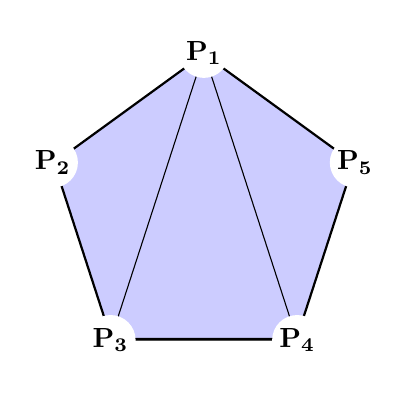
\begin{tikzpicture}
    % Draw the regular pentagon
    \node[regular polygon, regular polygon sides=5, shape border rotate=0, fill=blue!20, minimum size=4cm, thick, draw] (Pentagon) {};

    % Define coordinates for the vertices
    \coordinate (P1) at (Pentagon.corner 1);
    \coordinate (P2) at (Pentagon.corner 2);
    \coordinate (P3) at (Pentagon.corner 3);
    \coordinate (P4) at (Pentagon.corner 4);
    \coordinate (P5) at (Pentagon.corner 5);

    % Connect the vertices to form triangles
    \draw (P1) -- (P3) -- (P4) -- cycle;

    % Optional: Label the vertices
    \foreach \i in {1, ..., 5}
        \node[fill=white, inner sep=1pt, circle] at (P\i) {\(\mathbf{P_\i}\)};

\end{tikzpicture}
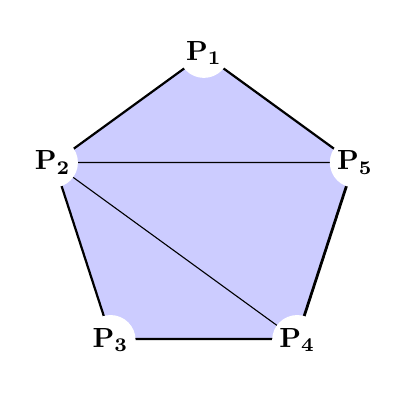
\begin{tikzpicture}
    % Draw the regular pentagon
    \node[regular polygon, regular polygon sides=5, shape border rotate=0, fill=blue!20, minimum size=4cm, thick, draw] (Pentagon) {};

    % Define coordinates for the vertices
    \coordinate (P1) at (Pentagon.corner 1);
    \coordinate (P2) at (Pentagon.corner 2);
    \coordinate (P3) at (Pentagon.corner 3);
    \coordinate (P4) at (Pentagon.corner 4);
    \coordinate (P5) at (Pentagon.corner 5);

    % Connect the vertices to form triangles
    \draw (P2) -- (P4) -- (P5) -- cycle;

    % Optional: Label the vertices
    \foreach \i in {1, ..., 5}
        \node[fill=white, inner sep=1pt, circle] at (P\i) {\(\mathbf{P_\i}\)};

\end{tikzpicture}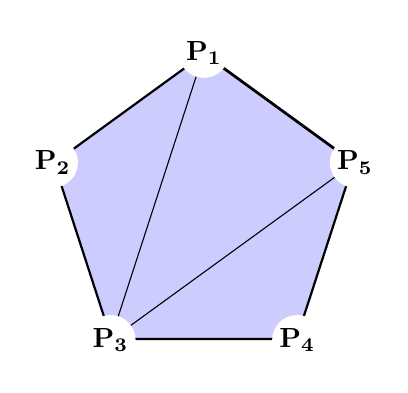
\begin{tikzpicture}
    % Draw the regular pentagon
    \node[regular polygon, regular polygon sides=5, shape border rotate=0, fill=blue!20, minimum size=4cm, thick, draw] (Pentagon) {};

    % Define coordinates for the vertices
    \coordinate (P1) at (Pentagon.corner 1);
    \coordinate (P2) at (Pentagon.corner 2);
    \coordinate (P3) at (Pentagon.corner 3);
    \coordinate (P4) at (Pentagon.corner 4);
    \coordinate (P5) at (Pentagon.corner 5);

    % Connect the vertices to form triangles
    \draw (P3) -- (P5) -- (P1) -- cycle;

    % Optional: Label the vertices
    \foreach \i in {1, ..., 5}
        \node[fill=white, inner sep=1pt, circle] at (P\i) {\(\mathbf{P_\i}\)};

\end{tikzpicture}
\]
\[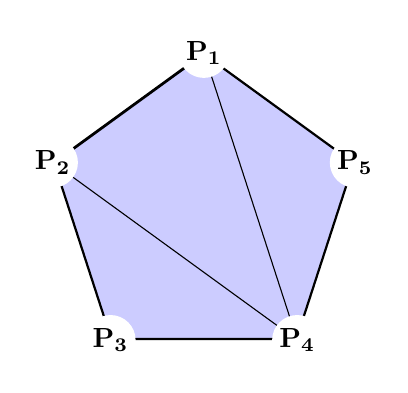
\begin{tikzpicture}
    % Draw the regular pentagon
    \node[regular polygon, regular polygon sides=5, shape border rotate=0, fill=blue!20, minimum size=4cm, thick, draw] (Pentagon) {};

    % Define coordinates for the vertices
    \coordinate (P1) at (Pentagon.corner 1);
    \coordinate (P2) at (Pentagon.corner 2);
    \coordinate (P3) at (Pentagon.corner 3);
    \coordinate (P4) at (Pentagon.corner 4);
    \coordinate (P5) at (Pentagon.corner 5);

    % Connect the vertices to form triangles
    \draw (P4) -- (P1) -- (P2) -- cycle;

    % Optional: Label the vertices
    \foreach \i in {1, ..., 5}
        \node[fill=white, inner sep=1pt, circle] at (P\i) {\(\mathbf{P_\i}\)};

\end{tikzpicture}
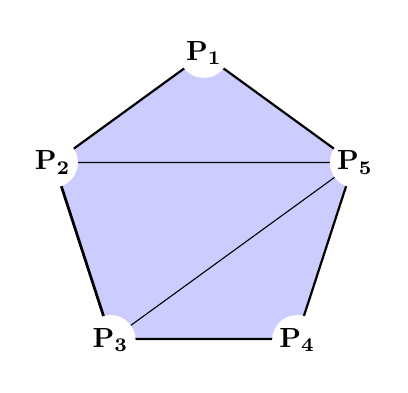
\begin{tikzpicture}
    % Draw the regular pentagon
    \node[regular polygon, regular polygon sides=5, shape border rotate=0, fill=blue!20, minimum size=4cm, thick, draw] (Pentagon) {};

    % Define coordinates for the vertices
    \coordinate (P1) at (Pentagon.corner 1);
    \coordinate (P2) at (Pentagon.corner 2);
    \coordinate (P3) at (Pentagon.corner 3);
    \coordinate (P4) at (Pentagon.corner 4);
    \coordinate (P5) at (Pentagon.corner 5);

    % Connect the vertices to form triangles
    \draw (P5) -- (P2) -- (P3) -- cycle;

    % Optional: Label the vertices
    \foreach \i in {1, ..., 5}
        \node[fill=white, inner sep=1pt, circle] at (P\i) {\(\mathbf{P_\i}\)};
\end{tikzpicture}\]

Thus, because there are $5$ ways to triangulate a polygon, then there are $5$ ways to rearrange the parenthesis.
}
\ex{For the $n=5$ case, consider a hexagon:\newline
There are two possible combinations of this triangulation:
\[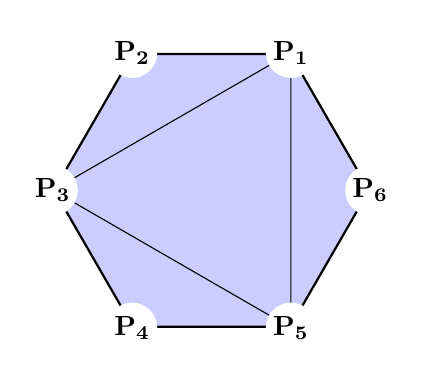
\begin{tikzpicture}
    % Draw the regular pentagon
    \node[regular polygon, regular polygon sides=6, shape border rotate=0, fill=blue!20, minimum size=4cm, thick, draw] (Hexagon) {};

    % Define coordinates for the vertices
    \coordinate (P1) at (Hexagon.corner 1);
    \coordinate (P2) at (Hexagon.corner 2);
    \coordinate (P3) at (Hexagon.corner 3);
    \coordinate (P4) at (Hexagon.corner 4);
    \coordinate (P5) at (Hexagon.corner 5);
    \coordinate (P6) at (Hexagon.corner 6);
    % Connect the vertices to form triangles
    \draw (P1) -- (P5) -- (P3) -- (P1) --cycle;

    % Optional: Label the vertices
    \foreach \i in {1, ..., 6}
        \node[fill=white, inner sep=1pt, circle] at (P\i) {\(\mathbf{P_\i}\)};
\end{tikzpicture}\]
$6$ possible combinations of this triangulation:
\[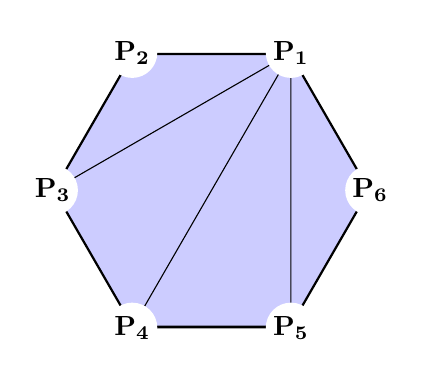
\begin{tikzpicture}
    % Draw the regular pentagon
    \node[regular polygon, regular polygon sides=6, shape border rotate=0, fill=blue!20, minimum size=4cm, thick, draw] (Hexagon) {};

    % Define coordinates for the vertices
    \coordinate (P1) at (Hexagon.corner 1);
    \coordinate (P2) at (Hexagon.corner 2);
    \coordinate (P3) at (Hexagon.corner 3);
    \coordinate (P4) at (Hexagon.corner 4);
    \coordinate (P5) at (Hexagon.corner 5);
    \coordinate (P6) at (Hexagon.corner 6);
    % Connect the vertices to form triangles
    \draw (P3)--(P1) -- (P5) -- (P4) -- (P1) --cycle;

    % Optional: Label the vertices
    \foreach \i in {1, ..., 6}
        \node[fill=white, inner sep=1pt, circle] at (P\i) {\(\mathbf{P_\i}\)};
\end{tikzpicture}\]
and $6$ more combinations of this triangulation:
\[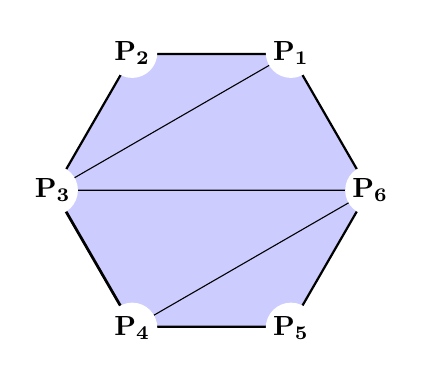
\begin{tikzpicture}
    % Draw the regular pentagon
    \node[regular polygon, regular polygon sides=6, shape border rotate=0, fill=blue!20, minimum size=4cm, thick, draw] (Hexagon) {};

    % Define coordinates for the vertices
    \coordinate (P1) at (Hexagon.corner 1);
    \coordinate (P2) at (Hexagon.corner 2);
    \coordinate (P3) at (Hexagon.corner 3);
    \coordinate (P4) at (Hexagon.corner 4);
    \coordinate (P5) at (Hexagon.corner 5);
    \coordinate (P6) at (Hexagon.corner 6);
    % Connect the vertices to form triangles
    \draw (P3)--(P4)--(P6) -- (P3) -- (P1) --cycle;

    % Optional: Label the vertices
    \foreach \i in {1, ..., 6}
        \node[fill=white, inner sep=1pt, circle] at (P\i) {\(\mathbf{P_\i}\)};
\end{tikzpicture}\]
Thus, $C_5 = 14.$}

\thm{Catalan Numbers Formula}{\[C_{n-1} = \sum_{i + j = n-1}C_iC_j\]}
\pf{
\[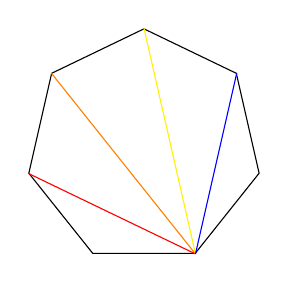
\begin{tikzpicture}
    % Draw a hexagon
    \node[regular polygon, regular polygon sides=7, minimum size=3cm, draw] (hectagon) {};

    % Draw the triangulation with colored lines
    \draw[orange] (hectagon.corner 2) -- (hectagon.corner 5);
    \draw[red] (hectagon.corner 3) -- (hectagon.corner 5);
    \draw[yellow] (hectagon.corner 1) -- (hectagon.corner 5);
    \draw[blue] (hectagon.corner 7) -- (hectagon.corner 5);
\end{tikzpicture}\]
One can create different polygons with each different line, so for example, with the red line, $C_5,$ then with the orange, and so on and on.
}

\newcommand{\calF}{\mathcal{F}}
\newcommand{\Sym}{\text{Sym}}

\chapter{Lecture 4- Symmetries of Shapes and Modulo Arithmetic}

\section{Symmetries}

\defn{A figure}{A figure $\calF$ is a subset of $\bbR^2.$ $\calF \subset \bbR^2.$}
\ex{$\triangle$}
\defn{Symmetry}{A symmetry is defined as $\Sym(\calF) = \{f \in \Isom(\bbR^2) | f(\calF) = \calF\}$
}
\defn{Subgroup}{We define $H$ to be a group, $G,$ if:
\begin{enumerate}
    \item $e \in H.$
    \item For all $h_1,h_2 \in H,$ $h_1 * h_2 \in H.$
    \item For all $h \in H,$ there exists a $h^{-1} \in H.$
\end{enumerate}}
\rmkb{Note that symmetries are subgroups of $\Isom(\bbR^2).$}
\ex{Various symmetries:
\begin{enumerate}
    \item $|\Sym(\triangle)| = 6.$
    \item $|\Sym(\square)| = 8.$
    \item $\Sym(\text{rectangle}) = 4.$
    \item $\Sym(\text{pentagon}) = 10.$
\end{enumerate}
}

But how do we prove, say, that $\Sym(\triangle) = 6?$ Consider the following reference: \[\begin{tikzpicture}
  % Define the points of the triangle
  \coordinate (A) at (0,0);
  \coordinate (B) at (4,0);
  \coordinate (C) at (2,3);

  % Draw the triangle
  \draw (A) -- (B) -- (C) -- cycle;

  % Label the vertices
  \node at (A) [left] {A};
  \node at (B) [right] {B};
  \node at (C) [above] {C};
  \node at (2,1.15) {O};
\end{tikzpicture}\] The key is that any symmetry, $f(\triangle) = \triangle,$ will send vertices to vertices, that is $f(\{A,B,C\}) = \{A,B,C\}.$ That is to say, $f$ is a bijection from $\{A,B,C\}$ to itself, and so it permutes $\{A,B,C\}.$ Therefore, we can construct a map \[\varphi: \Sym(\triangle) \to \bbS_n\], where $\bbS_3$ is defined as in Theorem 2.1.3.
\prop{$\varphi:\Sym(\triangle) \to \bbS_n$ is an isomorphism}
\pf{
\begin{enumerate}
    \item To first show that $\varphi$ is a homomorphism, that is, $\varphi(g_1 * g_2) = \varphi(g_1) * \varphi(g_2),$ it is obvious that the composition of symmetries is the same as the symmetry of compositions.
    \item To show that $\varphi$ is surjective, consider first the space of all possible ways to permute $\bbS_3:$
    \[\left(\begin{array}{ccc} 
    A & B & C\\
    A & B & C\\
    & \varphi(\text{Id}) &
    \end{array}\right) \qquad
    \left(\begin{array}{ccc} 
    A & B & C\\
    A & C & B\\
    & \varphi(\bbS_{OA}) &
    \end{array}\right) \qquad
    \left(\begin{array}{ccc} 
    A & B & C\\
    B & A & C\\
    & \varphi(\bbS_{OC}) &
    \end{array}\right)\]\[
    \left(\begin{array}{ccc} 
    A & B & C\\
    B & C & A\\
    & \varphi(R_O^{240^\circ}) &
    \end{array}\right) \qquad
    \left(\begin{array}{ccc} 
    A & B & C\\
    C & A & B\\
    & \varphi(R_O^{120^\circ}) &
    \end{array}\right)\qquad
    \left(\begin{array}{ccc} 
    A & B & C\\
    C & B & C\\
    & \varphi(\bbS_{OC}) &
    \end{array}\right)
    \] And thus, because every permutation has some symmetry relating to it, then $\varphi$ is surjective.
    \item Before proving that $\varphi$ is injective, it will be helpful to prove a little lemma and a corollarly:
    \lem{}{If $A,B,C \in \bbR^2$ are not on the same line and $f\in \Isom(\bbR^2)$ such that $f(A) = A,$ $f(B) = B,$ and $f(C) = C,$ then $f = \text{Id}$}
    \pf{Consider two circles of the same size, $C_1$ and $C_2,$ who's centers are at $A$ and $B,$ respectively. Consider then a third circle at $C,$ $C_3,$ that is a bit bigger. Then let $x \in C_1 \cap C_2 \cap C_3,$ and because $f \in \Isom(\bbR^3,),$ then it preserves distances, and so $f(x)\in C-1 \cap C_2 \cap C_3.$ Consider just $C_1$ and $C_2,$ if they touch at just one point, then it is impossible for $f(x)$ to be such point, since $C_C$ doesn't intersect the circle as both points. If they touch at all points, then $C_1 = C_2$ and so $A = .$ Therefore, they must touch at two points and $f(x) =x$ with a geometric argument.}
    \cor{If $A,B,C \in \bbR^2$ are not on the same line and $f,g\in \Isom(\bbR^2)$ such that $f(A) = g(A),$ $f(B) = g(B),$ and $f(C) = g(C),$ then $f = g$}
    \pf{Consider that $f(A) = g(A),$ and so $fg^{-1}(A) = A,$ and the same for the rest, and so by the lemma, $fg^{-1} = Id,$ and thus $f = g.$}
    Thus, back to the proof: Suppose $\varphi(g_1) = \varphi(g_2)$, then by the corollary above, $g_1 = g_2,$ and so $\varphi$ is injective.
\end{enumerate}
} 

However, this bijection does not hold for something like a square! Specifically, the surjectiveness breaks down, since, for example, there exists the permutation of vertices $\{A,B,C,D\}$ into vertices $\{A,B,D,C\},$ but that is impossible as a symmetry, as is clear by just trying to think of a symmetry which only change two verticies but not the other. 
\fact{A symmetry keeps vertices together}
\[\begin{tikzpicture}
  % Define the points of the triangle
  \coordinate (A) at (0,0);
  \coordinate (B) at (2,0);
  \coordinate (C) at (2,2);
  \coordinate (D) at (0,2)

  % Draw the triangle
  \draw (A) -- (B) -- (C) -- (D) -- cycle;

  % Label the vertices
  \node at (A) [left] {A};
  \node at (B) [right] {B};
  \node at (C) [above] {C};
  \node at (D) [above] {D};
  \node at (1,1) {O};
\end{tikzpicture}\]

\thm{$\Sym(P_n) = 2n$}{A regular polygon has $2n$ symmetries, were $n$ is the number of vertices of a polygon.}
\pf{Consider that a symmetry, $f,$ must send $f(A_i) = \{A_1, A_2, \dots, A_n\}.$ Therefore, if $A_1 = A_k,$ then, by the fact above, either:
\begin{enumerate}
    \item $f(A_2) = A_{k-1}$ and $f(A_n) = A_{k+1}$
    \item $f(A_2) = A_{k+1}$ and $f(A_n) = A_{k-1}$
\end{enumerate}
(Note that by the corollary above, this is enough to construct the symmetry)\newline
\begin{enumerate}
    \item In the second case, we are dealing with a rotation by $\frac{2\pi}{n}(k-1),$ or $R_O^{\frac{2\pi}{n}(k-1)}.$ 
    
    \[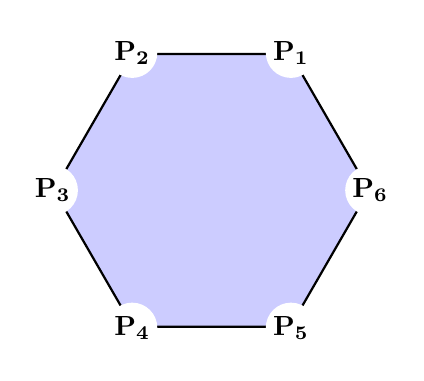
\begin{tikzpicture}
    % Draw the regular pentagon
    \node[regular polygon, regular polygon sides=6, shape border rotate=0, fill=blue!20, minimum size=4cm, thick, draw] (Hexagon) {};

    % Define coordinates for the vertices
    \coordinate (P1) at (Hexagon.corner 1);
    \coordinate (P2) at (Hexagon.corner 2);
    \coordinate (P3) at (Hexagon.corner 3);
    \coordinate (P4) at (Hexagon.corner 4);
    \coordinate (P5) at (Hexagon.corner 5);
    \coordinate (P6) at (Hexagon.corner 6);
    % Connect the vertices to form triangles

    % Optional: Label the vertices
    \foreach \i in {1, ..., 6}
        \node[fill=white, inner sep=1pt, circle] at (P\i) {\(\mathbf{P_\i}\)};
\end{tikzpicture} \xrightarrow[]{R_O^{\frac{2\pi (3) }{n}}}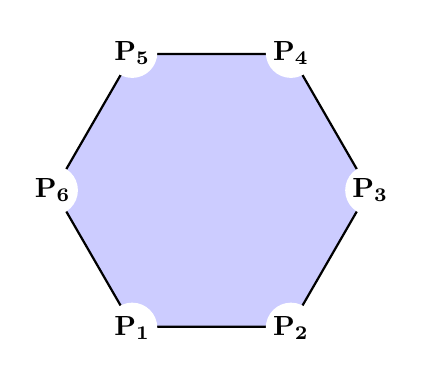
\begin{tikzpicture}
    % Draw the regular pentagon
    \node[regular polygon, regular polygon sides=6, shape border rotate=0, fill=blue!20, minimum size=4cm, thick, draw] (Hexagon) {};

    % Define coordinates for the vertices
    \coordinate (P4) at (Hexagon.corner 1);
    \coordinate (P5) at (Hexagon.corner 2);
    \coordinate (P6) at (Hexagon.corner 3);
    \coordinate (P1) at (Hexagon.corner 4);
    \coordinate (P2) at (Hexagon.corner 5);
    \coordinate (P3) at (Hexagon.corner 6);
    % Connect the vertices to form triangles

    % Optional: Label the vertices
    \foreach \i in {1, ..., 6}
        \node[fill=white, inner sep=1pt, circle] at (P\i) {\(\mathbf{P_\i}\)};
\end{tikzpicture}\]
\item In the second case, we can think of it as the same rotation as the first case, and then a symmetry across the $A_k$ line:
\[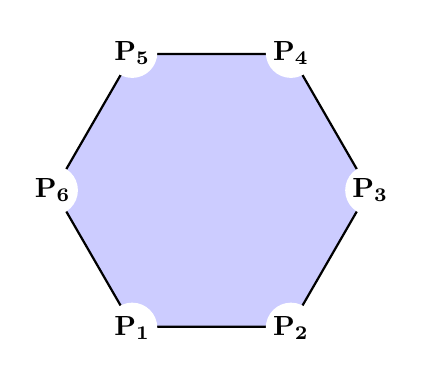
\begin{tikzpicture}
    % Draw the regular pentagon
    \node[regular polygon, regular polygon sides=6, shape border rotate=0, fill=blue!20, minimum size=4cm, thick, draw] (Hexagon) {};

    % Define coordinates for the vertices
    \coordinate (P4) at (Hexagon.corner 1);
    \coordinate (P5) at (Hexagon.corner 2);
    \coordinate (P6) at (Hexagon.corner 3);
    \coordinate (P1) at (Hexagon.corner 4);
    \coordinate (P2) at (Hexagon.corner 5);
    \coordinate (P3) at (Hexagon.corner 6);
    % Connect the vertices to form triangles

    % Optional: Label the vertices
    \foreach \i in {1, ..., 6}
        \node[fill=white, inner sep=1pt, circle] at (P\i) {\(\mathbf{P_\i}\)};
\end{tikzpicture} \xrightarrow[]{S_{OA_K}}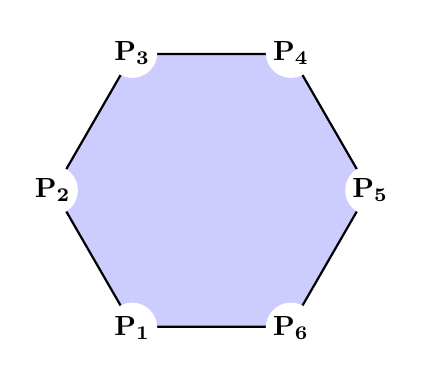
\begin{tikzpicture}
    % Draw the regular pentagon
    \node[regular polygon, regular polygon sides=6, shape border rotate=0, fill=blue!20, minimum size=4cm, thick, draw] (Hexagon) {};

    % Define coordinates for the vertices
    \coordinate (P4) at (Hexagon.corner 1);
    \coordinate (P3) at (Hexagon.corner 2);
    \coordinate (P2) at (Hexagon.corner 3);
    \coordinate (P1) at (Hexagon.corner 4);
    \coordinate (P6) at (Hexagon.corner 5);
    \coordinate (P5) at (Hexagon.corner 6);
    % Connect the vertices to form triangles

    % Optional: Label the vertices
    \foreach \i in {1, ..., 6}
        \node[fill=white, inner sep=1pt, circle] at (P\i) {\(\mathbf{P_\i}\)};
\end{tikzpicture}\]
\end{enumerate}
Thus, because we can do these two symmetries for any $i  \in [n],$ then we get $2n$ symmetries.
}

Now, think of a cube, which has $48$ symmetries, however, only $24$ of which are \textit{orientation preserving} (symmetries not due to reflections). This is $4!,$ which makes sense, since we are reflecting across the inner diagonals.

\section{Modulo Arithmetic}
\thm{Division with Remainder Theorem}{Let $a,b \in \bbZ,$ then there exists unique $q,r \in \bbZ$ such that:
\[a = qb + r \qquad 0\leq r \leq |b|\]}
\pf{:\\
\begin{enumerate}
    \item Existence: Let $A = \{a - qb \in \bbZ| a-qb \geq 0\} \neq \emptyset.$ By the Minimal Element Principle, since every subset of the integers contains its infemum, then let $r = \inf(A) \in A.$ Thus:
    \[r = a-qb \implies a = qb + r\] Assume that $r\geq |b|:$
    \begin{enumerate}
        \item If $b>0,$ then $r-b \in A$
        \item If $b<0,$ then $r + b \in A$
    \end{enumerate}
    which is a contradiction because both those terms are less than $r,$ the minimum term of $A.$
    \item Uniqueness:
    Let $a = q_1b + r_1$ and $a = q_2b + r_2,$  (where $0\leq r_1,r_2 \leq |b|).$ Then $q_1b+r_1 = q_2b + r_2,$ and thus $|q_1 - q_2|b = |r_2 - r_1|.$ Note that this is possible if an only if $|q_1 - q_2| = 0,$ which implies that $q_1 = q_2$ and $r_1 = r_2.$)
\end{enumerate}
}

\defn{Congruency Classes}{If $a,b \in \bbZ,$ then we say that $a \underset{n}{\equiv} b$ if $n | a-b$ if and only if there exists a $q\in \bbZ$ such that $a-b = qn.$}
\rmkb{We denote the class containing $a$ by $[a]$}
\ex{In $\bbZ / 5n\bbZ = [[0], [1], [2], [3], [4]].$ }


\chapter{Lecture 5- Orientation Preserving Symmetries with $\bbZ / n\bbZ$ and Complex Numbers}
\section{Orientation Preserving Symmetries}
\defn{A cyclic group of order $n$}{$\Sym^+(\bbP_n) = \{R_O^{\frac{2\pi}{n}k} | 0< k  < n-1\}$}

\lem{}{If $a \underset{n}{\equiv} b$ and $c \underset{n}{\equiv} d,$ then:
\begin{enumerate}
    \item $a+ b \underset{n}{\equiv} c + d.$
    \item $a-c \underset{n}{\equiv} b-d.$
    \item $ac \underset{n}{\equiv} bd.$
    \item $ka \underset{n}{\equiv} kb.$
    \item $a^k \underset{n}{\equiv} b^k$
\end{enumerate}}
\pf{:\\
2) $(a-b) = q_1n \qquad (b-d)  = q_2n,$ and thus $(a-b) - (c-d) = (q_1 - q_2)n,$ and thus $(a-b) \underset{n}{\equiv} (c-d).$\newline\newline
3) $ac \cdot bd = (q_1n +b)(q_2n +d) - bd = n[q_1q_2n + bq_2 + dq_1].$
}

\ex{
What are the last digits of:
\begin{enumerate}
    \item $9^{100}.$ Notice that $ 9 \underset{10}{\equiv} -1,$ and thus by the lemma, $9^{100} \underset{10}{\equiv}-1^{100} = 1.$
    \item $2^{300}.$ Notice that \[\begin{array}{cccccccc}
        2^0 & 2^1 & 2^2 & 2^3 & 2^4 & 2^5 & 2^7 & 2^8  \\
        1 &   2 & 4 & 8 & 6 & 2 & 4 & 8 & 
    \end{array}\] and thus consider that $300\mod 4 = 0,$ and thus it is the first one in the sequence, which is $6.$
\end{enumerate}
}

\defn{}{If $[a], [b] \in \bbZ / n\bbZ,$ then:
\begin{enumerate}
    \item $[a]+  {b} = [a+b].$
    \item $[a] - [b] = [a-b].$
    \item $[a]\cdot [b] = [ab].$
\end{enumerate}
}

\defn{Ring}{A \textit{ring} is has the same axioms as a field, except without there is no inverse required axiom.}
\ex{\begin{enumerate}
    \item $\bbZ.$
    \item $\bbZ/n\bbZ$ is a ring without inverses for non-prime $n.$
\end{enumerate}}

Define $\varphi: \bbZ / n\bbZ \to \Sym^+(P_n)$ such that if $[k]\in \bbZ/n\bbZ,$ then $\varphi([k]) \to R_O^{\frac{2\pi k}{n}}$
\prop{$\varphi$ is an isomorphism}
\pf{:\\
\begin{enumerate}
    \item $\varphi$ is obviously surjective.
    \item $\varphi$ is injective because $|\bbZ/n\bbZ| = |\Sym(P_n)|.$
    \item $\varphi$ is a homomorphism because:
    \[\varphi([k_1] + [k_2]) = \varphi([k_1+ k_2]) = R_O6[\frac{2\pi}{n}(k_1 + k_2) = R_O^{\frac{2\pi k_1}{n}}\circ R_O^{\frac{2\pi k_2}{n}} \]
\end{enumerate}}

\section{Complex Numbers}
\defn{Complex Numbers}{The \textit{complex numbers} are defined as $\bbC = \bbR^2\{(a,b) \in \bbR^2\}.$ Multiplication and addition is defined as follows:
\[(a,b) + (c,d) = (a+c, b + d)\]
\[(a,b)(c,d) = (ac -bd, ad -bc\]}
\begin{figure}[h!]
    \centering
    \includegraphics[width=0.5\linewidth]{REU-2024//Images/image.png}
    \caption{Complex Plane}
\end{figure}
\rmkb{A complex number, $(a,b),$ is usually denoted by $z = (a,b) = a+bi.$}
\rmkb{One can check to verify that $\bbC$ is indeed a field.}
\thm{$i^2 = 1$}{We denote $i = (0,1).$ Thus, by definition:
\[i^2 = (0,1)(0,1) = (-1, 0) = -1\]}
\rmkb{Note that the only tricky axiom to check in the above remark is the inverse one, as division is tricky with complex numbers. However, as long as $a^2 + b^2 \neq 0,$ then we can write $(a+bi)(\frac{a-bi}{a^2 + b^2}) = 1$}
\defn{|z| and $\arg(z)$}{\[r = |z| = \sqrt{a^2 + b^2}\]
\[\phi = \angle  = \arg(z)\]}
\prop{$a = |z|\cos(\varphi), b = |z|\sin(\varphi)$, and thus $z = a+bi = |z|(\cos(var\phi) + i\sin(\varphi)).$}

\fact{\begin{enumerate}
    \item $|z_1 \cdot z_2| = |z_1|\cdot |z_2|$
    \item $\arg(z_1z_2) = \arg(z_1) + \arg(z_2).$
\end{enumerate}}
\rmk{Multiplying complex numbers scales them by multiplying their magnitudes and adds the angles.}
\defn{Conjugate Complex Number}{Given $z = a+bi \in \bbC,$ we define its \textit{conjugate}, $\overline{z}, $ to be $\overline{z} = a-bi.$}
\cor{$\overline{z_1} + \overline{z_2} = \overline{z_1 + z_2}$\newline
$\overline{z_1}\cdot \overline{z_2} = \overline{z_1z_2}$}

\lem{Powers}{$(\cos(\varphi) + i\sin(\varphi))^n = cos(n\phi) + i\sin(n\phi)$}
\pf{Apply the above remark $n$ times}
\defn{Exponents}{We define $e^{i\varphi}= \cos(\varphi) + i\sin(\varphi)$}
\rmkb{From this, we get the identity that:
\[\cos(x) = \frac{e^{ix} + e^{-ix}}{2}\qquad \cos(x) = \frac{e^{ix} - e^{-ix}}{2i}\]}
\lem{Euler's Identity}{$e^{i\pi} = -1$}
\section{A Complex Isometry}
\thm{All complex isometries}{Let $f: \bbC \to \bbC$ be a function. $f(z) = mz +b$ is an isometry if an only if $|m=1|.$}
\pf{Let $f(z) = w.$ This is only possible if and only if $z = \frac{w-b}{m}.$ Note that because an explicit inverse formula was given, then $f$ is a bijection. Moreover, \[|f(z_1)- f(z_2)| = |mz_1 + b - mz_2 -b| = |m(z_1 - z_2)| = |z_1 - z_2|.\]}

\thm{All $\bbR^2$ isometries}{Any isometry $f: \bbR^2 \to \bbR^2$ is either $z = mz + b$ or $z = m\overline{z} + b$ for $|m|=1$.}
\ex{
\begin{enumerate}
    \item $z \to z + b\hfill (T_b).$
    \item $z\to -z\hfill (S_O).$
    \item $z\to mz \hfill (R_O^\phi).$
    \item $z \to \overline{z}\hfill (\bbS_\bbR).$
\end{enumerate}
}

\chapter{Lecture 6- Roots of Unity and Classifications of Isometries}
\section{Roots of Unity}
\thm{Fundamental Theorem of Algebra}{If $P(x)$ is a polynomial ($P(x) \in \bbP[x]),$ then it has a complex root}
\ex{Consider $x^n - a = 0$. Let \[a = r(\cos(\varphi) + i\sin(\varphi))\qquad x = R((\cos(\Theta) + i\sin(\Theta))\] It is evident that $R = \sqrt{n}$ and $\Theta = \frac{\varphi}{n} + 2\pi\frac{k}{n},$ for $0\leq k\leq n-1.$}
\ex{With the same example as above, consider $a = 1.$ Then if $\varepsilon_k = \cos(\frac{2\pi k}{n}) + i\sin(\frac{2\pi k}{n}) = e^{\frac{2\pi i k}{n}},$ then $\mu_0 = \{\varepsilon_0, \varepsilon_1, \dots, \varepsilon_{n-1}\}$ are the verticices of $n-$regular polygons }
\begin{figure}
    \centering
    \includegraphics[width=0.5\linewidth]{REU-2024//Images/unity.png}
    \caption{Roots of Unity}
\end{figure}
\ex{If $n=3,$ then $x^{3} - 1=0,$ and so $(x-1)(x^2 + x + 1) = 0,$ and thus $x = \{1, \frac{-1\pm \sqrt{3}}{2}\}$}

\thm{}{$\bbZ/n\bbZ$ is isomorphic to $\mu_n.$}
\pf{Let $\varphi: [k] \to \varepsilon_k.$
\begin{enumerate}
    \item \[\varepsilon_k \varepsilon_\ell= (\cos(\frac{2\pi k}{n}) + i\sin(\frac{2\pi k}{n}))(\cos(\frac{2\pi \ell}{n}) + i\sin(\frac{2\pi \ell}{n})) = \cos(\frac{2\pi (k+\ell)}{n}) + i\sin(\frac{2\pi (k + \ell)}{n}) = \varepsilon_{k+\ell}\]
    \item This is obviously bijective since $|\mu_0| = |\bbZ/n\bbZ|.$
\end{enumerate}}

\thm{Classifications of Isometries}{Every isometry $f: \bbC \to \bbC$ is one of the following:
\begin{enumerate}
    \item $z \to mz + b$ (orientation-preserving).
    \item $z\to m\overline{z} + b$ (orientation-reversing).
\end{enumerate}}
\pf{Let $f$ be an isometry and consider $f(0)$, $f(1),$ and $f(i).$ Define $f_1(z) = f(z) - f(0),$ and notice that \begin{align*}
    f_1(0) &= 0\\
    f_1(1) &= 1 \implies |1-0| = |f_1(1) - f_1(0)| = |f_1(1)|= 1\\
\end{align*} Define:
    \[f_2(z)= \frac{f(z) - f(0)}{f(1) - f(0)}\implies f(0) = 0, \quad f(1) = 1\]
Thus, there are two cases:
\begin{enumerate}
    \item If $z = \frac{f(z) - f(0)}{f(1) - f(0)},$ then $f(z) = (f(1) - f(0))z + f(0).$
    \item If $\overline{z} = \frac{f(z) - f(0)}{f(1) - f(0)},$ then $f(z) = (f(1) - f(0))\overline{z} + f(0).$
\end{enumerate}
    }

\thm{Classification of Orientation Preserving Isometries}{$\Isom(\bbR^2)$ is a subgroup, and every element in $\Isom^+$ is either:
\begin{enumerate}
    \item An identity.
    \item A translation.
    \item A rotation.
\end{enumerate}}
\pf{
\begin{enumerate}
    \item Consider that if $f_1, f_2 \in \Isom^+(\bbR^2),$ then $f_1 \circ f_2 = m((m)z + b')+ b' = mm'z + (m'b + b'),$ $f_I = f(z) = mz,$ $m=1.$
    \item $f(z) = z + b$ is a translation.
    \item $f(z) = mz + b$ is a rotation, with a fixed point at $z_0 = \frac{b}{1-m}$
\end{enumerate}
}
\thm{Chasle's Theorem}{Every isometry $f: \bbR^2 \to \bbR^2$ is one of the following:
\begin{enumerate}
    \item Identity
    \item Rotation
    \item $T_{\textbf{v}}$
    \item $\bbS_{\ell}$
    \item $\bbS_{\ell}T_{\textbf{v}}$
\end{enumerate}}

\cor{\[R_{O_1} ^ {\varphi_1} \circ R_{O_2} ^ {\varphi_2} = \begin{cases}
    R_{O_3} ^ {\varphi_1 + \varphi_3} \qquad \varphi_1 + \varphi_2 \neq 2\pi k\\
    T_{\textbf{v}} \qquad \varphi_1 + \varphi_2 = 2\pi k
\end{cases}\]}

\pf{ Consider the following functions:
\[z\to e^{i\varphi_1}z + b_1\qquad z\to e^{i\varphi_2}z + b_2\]
and thus by multiplying, $e^{i(\varphi_1 + \varphi_2)z + (b_1 e^{i\varphi_2} + b_2)}.$
}
\newpage
\thm{Napoleon's Theorem}{Given a $\triangle ABC$ and creating equilateral triangles on each edge and having the center points be $O_A, O_B, O_C,$ then $\triangle O_AO_BO_C$ is a regular triangle.}
\begin{figure}[h!]
    \centering
    \includegraphics[width=0.5\linewidth]{REU-2024//Images/Napoleon's Theorem.png}
    \caption{Napoleon's Theorem}
\end{figure}
s
\defn{Similarities}{A function $f: \bbR^2 \to \bbR^2$ is a \textit{similarity} if there exists a $k \in \bbR$ such that for all $A,B \in \bbR^2,$ \[|f(A)f(B)| = k|AB|\]}
\ex{Given $H_O^\lambda: \bbR^2 \to \bbR^2,$ with $\lambda \neq 0$ such that $H_O^\lambda(X) = Y$ with $\lambda \overrightarrow{OX} = \overrightarrow{OY}$}

\chapter{Lecture 7- Fundamental Theorem of Arithmetic and Euler's Function for $\bbZ/n\bbZ.$}
\section{Prime Numbers and FTA.}
Recall the integer remained theorem:
\fact{For all $a,b \in \bbZ,$ with $b\neq 0,$ there exists unique $q, r \in \bbZ$ such that $a = qb + r$ and $0\leq r \leq |b|.$}
\rmkb{We say that $b|a$ if and only if there exists a $q\in \bbZ$ such that $a = bq.$ Moreover, we say that $a_1\underset{n}{\equiv} a_2$ if and only if $n | (a_1 - a_2)$ }
\defn{Greatest Common Divisor}{The \textit{greatest common divisor}, or \textit{gcd}, between $a,b \in \bbZ,$ is $\gcd(a,b) = (a,b) = \max\{d \in \bbN | d | a, d|b\}$}
\prop{\begin{enumerate}
    \item $(a,b) = (a-b, b).$
    \item $(a,b) = (b,a).$
    \item $(3,0) = 3.$
\end{enumerate}}

\thm{Euclid's Algorithm}{\begin{enumerate}
    \item If $b  = 0,$ then $(a,b) = a.$
    \item Use fact 7.1.1 to write $(a,b) = (q_1b  + r_1, b) = (r_1, b) = (b,r_1).$ If $r_1 = 0,$ then $(a,b) = b.$
    \item Use fact 7.1.1 to write $(b,r_1) = (q_2r_1 + r_2,r_1),$ and keep going until $r_n = 0,$ and thus $(a,b) = r_{n-1}.$ Note that this process terminates eventually because integers eventually decrease down to $0.$
\end{enumerate}}
\cor{Suppose $a,b \in \bbZ$ with $(a,b) = d,$ then there exists $u,v \in \bbZ$ such that $d = ua + vb.$}
\pf{This comes from the fact that in Euclid's Algorithm, $d = \langle r_{n-1}, r_n\rangle,$ and so on and on.}
\ex{(31,22)
\begin{align*}
    (31,22) &= (9,22)\\
    &= (9,4)\\
    &= (1,4)
\end{align*}
And thus $(31,22) = 1.$ Moreover, we can write $1$ as
\[1 = 9-(2\cdot4) = (9 - 2\cdot (22 - 9\cdot 2)) = 5 \cdot 9 - 2\cdot 22 = 5(31 - 22) - 2(22) = 5(31) - 7(22)\]
}

\defn{Coprime}{We say that $a,b \in \bbZ$ are \textit{coprime}if $(a,b) = 1.$}
\rmkb{By the above corollary, $a,b\in \bbZ$ are coprime if and only if there exist $u,v \in \bbZ$ such that $1 = ua  + vb.$}
\defn{Prime}{We say that $p \in \bbN$ is prime if an only if $p$ has exactly two divisors, namely, $1$ and $p.$}
\thm{}{Every $n \in \bbZ$ is a product of primes}
\pf{induct}
\prop{There exists an infinite amount of prime numbers}
\pf{Assume there exists $N$ primes. Therefore, consider $a = p_1p_2\cdots p_N + 1.$ By the above theorem, there exists some $p_i$ prime such that $p_i| a.$ However, this is a contradiction, as any prime dividing $a$ would result with remainder $1.$}

\thm{}{For any $a \in \bbZ,$ either $p | a$ or $(p,a) = 1.$}
\thm{}{The following statements hold:
\begin{enumerate}
    \item If $ma \underset{n}{\equiv} m b$ and $(m,n) = 1,$ then $a\underset{n}{\equiv}b.$
    \item If $n | (ma)$ and $(m,n) = 1,$ then $n | a.$
    \item If $p | (ab),$ then $p|a$ or $p|b.$ 
\end{enumerate}}
\pf{
\begin{enumerate}
    \item Because $ma \underset{n}{\equiv} m b$ implies that $n | (a-b)m,$ then by (2), we have that $n | (a-b),$ and thus $a\underset{n}{\equiv} b$
    \item Because $(m,n) = 1,$ then \[1 = um + vn\quad \implies \quad a = uma + vna\] Because the RHS is divisible by $n$ ($n | (ma)$), then $n | a.$
    \item If $p|a,$ we are done. If not, assume $p\not| b,$ then we have, by Theorem 7.1.10, that $p|a,$ which is a contradiction.
\end{enumerate}
}

\thm{Fundamental Theorem of Arithmetic}{If $a\in \bbZ$ and $a \neq 0,$ then we can write $a = p_1^{n_1} \cdot p_2^{n_2}\cdots p_k^{n_k}$ in 1 distinct way (up to the ordering of the factors)}
\pf{\begin{enumerate}
    \item Already proven in Theorem 7.1.8.
    \item Assume \[a = p_1^{n_1} \cdot p_2^{n_2}\cdots p_k^{n_k} = s_1^{n_1} \cdot s_2^{n_2}\cdots s_k^{n_k}.\] If $q_s \notin \{p_1, \dots, p_k\},$ then $q_s$ is coprime with all $p.$ Because $q_s | p_1 \cdots p_k,$ then by Theorem 7.1.11.3, we are done.
\end{enumerate}}

\section{$\bbZ/n\bbZ$ Rings}
Recall that $\bbZ/n\bbZ$ is a ring. \newline
Define $R^* = \{x\in R | \exists y \in R ; xy = 1\}.$ Note that $R^*$ is therefore an Abelian Group.\rmkb{Note that $R$ is a field if and only if for all $x\in R$ such that $x\neq 0,$ we have that $x\in R^*.$}

\thm{When is $[a]$ Invertible?}{$[a]\in (\bbZ/n\bbZ)^*$ if and only if $(an) = 1,$ that is, $a,n$ coprime.}
\pf{Consider that $[a]$is invertible if and only if there exists a $[b] \in \bbZ/n\bbZ$ such that $[a][b] = 1,$ which exists if and only if there exists a $b$ such that $n| ((a-b)-1),$ which exists if an only if there exists $b,q \in \bbZ$ such that $(a-b)-1 = qn,$ and thus $1 = ab-qn.$}

\ex{What is $[22]^{-1}$ in $\bbZ/31\bbZ?$ Consider that $1 = 5(31) - 7(22),$ and thus $[1]= [5][31] - [7][22] = [-7][22],$ and so $[22]^{-1}= [-7] = [24].$}

\cor{\begin{enumerate}
    \item $|\bbZ/n\bbZ| = \varpi(n)$ (Euler's function). Note that $|\bbZ/p\bbZ| = p-1$ where $p$ is prime.
    \item $\bbZ/p\bbZ$ is a field.
\end{enumerate}}

\thm{Euler's Theorem}{Let $a \in \bbZ$ and $n\in \bbN$ such that $(a,n) = 1,$ then $a^{\varphi(n)} \underset{n}{\equiv} 1.$}

\pf{Suppose $(\bbZ/n\bbZ) = \{[a_1], [a_2], \dots, [a_{\varphi(n)}]\}.$\newline Let $A = \{[a][a_1], [a][a_2], \dots, [a][a_{\varphi(n)}]\}$. I claim that these are the same set, up to the order of the elements. This holds because (1) the first question on PSET 3 and (2) because for any $i\neq j \in [\varphi(n)],$ we have that $[a][a_i] = [a][a_j],$ then $[a_i] = [a_j].$ Therefore:
\[[a_1], [a_2], \dots, [a_{\varphi(n)}] = [a][a_1], [a][a_2], \dots, [a][a_{\varphi(n)}]\], and thus
\[[1] = [a]^{\varphi(n)}\]
}
\thm{Fermat's Last Theorem}{If $p$ is a prime and $(a,p) = 1,$ then $a^{p-1} \underset{p}{n} 1$}

\cor{(Wilson's Theorem) Let $p$ be a prime and $p\geq 3,$ then $(p-1)! \underset{n}{-1}.$}
\pf{Consider that \[[(p-1)!] = [p-1][p-2]\cdots [2][1] = [1][p-1] \prod_{1<x<p-1}[x][x]^{-1} = -1 \cdot 1\] Consider that $[x] = [x]^{-1}$ when $[x^2] = 1$ when $p | x^2 - 1,$ and thus $p | x-1$ or $p| x+1,$ and thus either $[x] = [1]$ or $[x] = -1.$ Therefore, the last equality holds.}

\chapter{Lecture 8- Fields and Polynomials, Inversions}
\section{Fields and Polynomials}
\ex{Examples of Fields:
\begin{enumerate}
    \item $\bbC, \bbR, \bbQ;$
    \item $\bbQ(\sqrt{2}) = \{a + b\sqrt{2} | a,b \in \bbQ\},$ where inverses are defined by multiplying by conjugates: $\frac{1}{a + b\sqrt{2}} = \frac{a-b\sqrt{2}}{a^2 - 2b^2}.$
    \item $\bbF_2.$
\end{enumerate}
}

\defn{Characteristics of Fields}{
\begin{enumerate}
    \item We say a field, $F,$ has \textit{characteristic zero} if \[\underbrace{1 + 1+ \cdots +1}_{\text{$n$ times}}\neq 0, \qquad \forall n\in \bbN\] 
    \rmkb{With such a field we can build an injective map $\bbQ \to F$ by sending \[\frac{n}{m} \to \underbrace{(1 + 1 + \dots + 1)^{-1}}_{\text{$m$ times}}\underbrace{(1 + 1 + \dots + 1)}_{\text{$n$ times}}\] Therefore, we get a notion of \textit{Inclusion of Fields}, which implies that a 'copy' of $\bbQ$ is found in every field of characteristic zero.}
    \item We say a field, $F,$ has \textit{characteristic p}, if there exists some $N\in \bbN$ such that \[\underbrace{1 + 1+ \cdots +1}_{\text{$n$ times}}= 0.\] 
    \rmkb{We know the smallest such $n$ must be prime, as otherwise, either factor of $n$ would be the one contributing the zero, which is a contradiction, since if its a factor, then its smaller than $n.$ Thus, we can build an injective map $\bbZ/p\bbZ\to F$ by sending 
    \[[k] \to \underbrace{1 + 1+ \cdots +1}_{\text{$k$ times}},\] and thus we get the notion that $\bbF_p \subset F.$}
\end{enumerate}
}

\thm{}{Suppose $F$ is a finite field, then $|F|^p = p^n$ for some $n\in \bbN$.}
\pf{$F$ cannot have characteristic $0,$ as it is finite, and thus $\text{char}(F) = p$ for some $p$ prime. Notice then that $F$ is a vector space of $\bbF_p,$ and we know also that because $\dim(F)<\infty,$ then $\dim(F) = n$ for some $n\in \bbN.$ Therefore, we know that $F \cong F_p^n,$ and thus $|F| = |F_p^n| = p^n.$}

\defn{Polynomial}{A \textit{polynomial} with coefficients in $F$ is a sequence $(a_0, a_1, \dots)$ with each $a_i \in F$ such that there exists some $N\in \bbN$ with all $n\geq N$ yielding $a_n = 0.$ Addition and multiplication are defined as follows:
\[+: ((a_0, a_1, \dots) + (b_0, b_1, \dots) = (a_0 + b_0, a_1 + b_1, \dots)\]
\[\times: (a_0, a_1, \dots) \times (b_0, b_1, \dots) = (a_0b_0, a_0b_1 + a_1b_0, \dots)\]
}
\fact{A polynomial is a ring}
\pf{While tedious, it is useful to note that the identity element is \[1 = (1,0,0,\dots),\] and to arrive at a usual notion of a polynomial, simply use the fact that:
\[x = (0,1,0\dots)\] and thus \[x^n = (\underbrace{0,0,\dots, 1}_{\text{$n+1$ times}},0,\dots)\]}
\newpage
\section{Inversions}
\defn{Inversion}{Let $S$ be a circle of radius $R$ and with a center at $O.$ Then we define as inversion to be the map $I_S: \bbR^2\sm\{O\} \to \bbR^2\sm\{O\}$ such that $I_S(X) = Y$ if:
\begin{enumerate}
    \item $Y\in$ line connecting $O,X.$
    \item $|OX||OY| = R^2.$
\end{enumerate}
}
\begin{figure}[h!]
    \centering
    \includegraphics[width=0.5\linewidth]{REU-2024//Images/Inversion.png}
    \caption{Inversion}
\end{figure}
\prop{
\begin{enumerate}
    \item Points on $S$ are fixed;
    \item Points inside of $S$ are mapped outside, and vice-versa;
    \item $I_S^2 = \text{Id};$
    \item If $A,B \in \bbR^2,$ then \[\frac{|OA}{OI(B)} = \frac{|OB|}{|OI(A)|}\] i.e, Figure 8.2 below;
    \item Lines containing $O$ are unchanged under inversions;
    \item Lines not containing $O$ are sent to circles with $A,B,O$ on the circle;
    \item Circles not containing $O$ are sent to circles containing $O.$
\end{enumerate}
}\begin{figure}[h!]
        \centering
        \includegraphics[width=0.5\linewidth]{REU-2024//Images/Triangle Inversion.png}
        \caption{Triangle Inversion}
    \end{figure}

\defn{Riemann Sphere}{A \textit{Riemann sphere}, or a \textit{projective line over $\bbC,$ is $\bbC \cup \{\infty\} = \Tilde{\bbC} = \bbP_\bbC'.$}}
\rmkb{A line in $\bbR^2$ is mapped to a line $\cup \{\infty\},$ and \[I_S(\infty) = 0,\qquad I_S(0) = \infty.\]}

\chapter{Lecture 9- Roots of Polynomials, Lagrange Interpolation, and Mobius Groups}
\section{Roots of Polynomials}
\thm{Polynomial Division with Remainder Theorem}{If $A(x), B(x)\in F[x],$ and $Q(x)\neq 0,$ then there exists unique polynomials $R(x), Q(x)$ such that $A(x) = Q(x)B(x) + R(x)$ and $0<\deg(R(x))< \deg(B(x)).$}
\pf{The proof follows exactly the same as Theorem 4.2.1, but just with polynomials and degrees.}

\defn{Roots}{Given that $P(x)\in F[x]$ and $x_0 \in F,$ we say that $x_0$ is a \textit{root} of $P(x)$ if $P(x_0) = 0.$}

\defn{Polynomial Divisions}{Suppose $A(x), B(x)\in P(x),$ then we say that $A(x) | B(x)$ if and only if there exists a $Q(x)\in F[x]$ such that $B(x) = A(x)B(x).$}

\lem{}{Suppose that $P(x)\in F[x],$ then $x_0\in F$ is a root of $P(x)$ if and only if $(x-x_0) | P(x).$}
\pf{
\begin{itemize}
    \item ($\implies:$) Divide $P(x)$ by $(x-x_0)$ with remainder. Then $P(x) = Q(x)(x-x_0) + R(x),$ and thus $P(x_0) = 0 = Q(x_0)(x_0 - x_0) + R(x),$ and thus $R(x) = 0,$ meaning that there is no remainder, and thus $(x-x_0) | P(x).$
    \item ($\impliedby:$) If $(x-x_0) | P(x),$ then $P(x)  = (x-x_0)Q(x),$ and thus, $P(x_0) = 0.$
\end{itemize}
}

\cor{:\\
\begin{enumerate}
    \item Suppose $P(x)\in F[x]$ and $\deg(P(x)) = n,$ then $P(x)$ has at most $n$ roots.
    \item If $P(x)\in F[x]$ has roots $x_1, \dots, x_n$ and is of degree $n,$ then we can write:
    \[P(x) = (x-x_1)P_1(x) = (x-x_0)(x-x_2)P_2(x) = \dots = a_n(x-x_1)\cdots(x-x_n)\]
    \item If $P(x) = a_n(x-x_1)\cdots(x-x_n),$ then 
    \[\frac{-a_{n-1}}{a_n} = x_1 + \dots + x_n, \qqiad  \frac{\pm a_{n-k}}{a_n} = \sum_{1<<k}x_1\cdots x_k,\qquad (-1)^n\frac{a_1}{a_n} = x_1 \cdots x_n\]
    \item Let $P(x),Q(x)\in F[x]$ and $\deg(P,Q) \leq n$ and let there exist $(n+1)$ distinct $x_1, \dots, x_{n+1} \in F$ such that $P(x_i) = Q(x_j),$ then $P = Q.$
\end{enumerate}
}
\pf{Proofs mostly use previous lemma.}

\thm{}{Let $F$ be an infinite field. If for all $a\in F,$ $P(a) = Q(a),$ then $P = Q.$}
\pf{Let $P,Q,$ have degree $n,$ then because there exists more than $n+1$ such $a\in F$ (since it is infinite), by the last part of the corollary, we are done.}

\section{Lagrange Interpolation}
\thm{Lagrange Interpolation Theorem}{Let $x_0, x_1, \dots, x_n$ and $y_0, y_1, \dots, y_n$ be elements of $F.$ Then There exists a unique $P(x)\leq F[x]$ such that $P(x_1) = y_1, \dots, P(x_n) = y_n$ of $\deg(P)<n-1$}
\rmkb{Intuitively, this says that if we have $n$ points, say $3,$ we can create a unique polynomial of degree $n-1$, say a quadratic, that passes through all those points}
\pf{
Uniqueness by Corollary. Consider 
\[P(x) = y_1 \frac{(x-x_2)(x-x_3)\cdots (x-x_n)}{(x_1 - x_2)(x_1 - x_3)\cdots(x_1 - x_n)} + y_2\frac{(x-x_1)(x-x_3)\cdots (x-x_n)}{(x_2 - x_1)(x_2 - x_3)\cdots(x_2 - x_n)} + \dots + y_n\frac{(x-x_1)(x-x_2)\cdots (x-x_{n-1})}{(x_n - x_1)(x_n- x_2)\cdots(x_n - x_{n-1})}\]
}
\ex{
Fermat's Little Theorem:
\begin{enumerate}
    \item \[\bbF_3: \qquad x^2-[1] = (x - [1])(x-[2])\]
    \item \[\bbF_5: \qquad x^4-[1] = (x - [1])(x-[2])(x - [3])(x - [4])\]
    \item \[\bbF_p: \qquad x^{p-1}-[1] = (x - [1])(x-[2])\cdots(x-[p-1])\]
\end{enumerate}
}

\section{Mobius Groups and Fractional Linear functions}

\defn{Mobius Group}{Consider the group of bijections $\bbP_\bbC'\to \bbP_\bbC',$ then we define a \textit{Mobius Group} to be the subgroup generated by $\Sym(\bbR^2)$ and inversions.}

\defn{Fractional Linear Functions}{A \textit{fractional linear function} is a map $f: \bbP_\bbC'\to \bbP_\bbC'
$ such that $f(z) = \frac{az  + b}{cz + d}$ given that $ad - bc\neq 0$ and 
\begin{enumerate}
    \item If $c = 0,$ then we have that $z\to \frac{az}{d} + \frac{b}{d}$ and $\infty \to \infty.$
    \item If $c\neq 0,$ then we have that $f(\frac{-d}{c}) = \infty$ and $f(\infty) = \frac{a}{c}.$
\end{enumerate}
}
\thm{}{Fractional linear functions form a group (denoted by $PGL_Q(\bbC).$)}

\newcommand{\ord}{\text{ord}}
\chapter{Lagrange's Theorem and The Gauss Theorem for Cyclic Groups}
\section{Lagrange's Theorem}
\thm{Lagrange's Theorem}{Let $G$ be a finite group and let $a\in G,$ then $a^{|G|} = e.$}
\cor{Fermat's Little Theorem: Consider any $a\in (\bbZ/p\bbZ)^*,$ then $[a]^{p-1} = [1]$ if and only if $p | a^{p-1}$}
\pf{Let $a\in G,$ and let $G = \{g_1, g_2, \dots, g_n\}.$ Consider a graph where $g_i \to g_j$ if there is an edge whenever $g_i = ag_j.$ Note that for every vertex, there exists a unique outgoing and incoming edge. Therefore, the group creates various loops. For example, $g_1, ag_1, a^2g_1, \dots, a^{k-1}g_1$ is a loop where each element is distinct and $a^kg_1 = g_1.$ Define
\[k: = \{S_{\geq 1} : a^S = e\}=: \ord(a)\], then $|G| = k(\#\text{cycles}),$ and thus $a^k = a^{|G|} = e$ for any $a\in G.$}
\cor{Let $a\in G$ and $G$ be finite, then $\ord(a) | |G|.$}
\cor{If $|G| = p,$ then $G \cong (\bbZ/p\bbZ, +)$}
\pf{The map sends $[k]\to a^k.$}
\section{Cyclic Groups and Gauss' Theorem}
\defn{Cyclic Groups}{A group $G$ is cyclic if it is generated by $1$ element, i.e, there exists an $a\in G$ such that for all $g\in G,$ $g$ is a power of $a.$}
\prop{If $G$ is cyclic, then either $G\cong (\bbZ, +)$ or $G\cong (\bbZ/n\bbZ, +)$}
\thm{Gauss' Theorem}{If $(\bbZ/p\bbZ)^*$ is cyclic, then it is isomorphic to $(\bbZ/(p-1)\bbZ, +).$}
\lem{}{Consider the cyclic group of order $n,$ $\bbZ/n\bbZ.$ Then there exists $\varphi(d)$ number of elements with order $d.$}
\pf{This proof is mostly done by exploring examples, but an important corollary is \[n = \sum_{d | n}\varphi(d)\]}
\pf{Proof for Gauss consists of showing that $\Psi(p-1)\neq0,$ where $\Psi$ is the number of elements of order $d$ in $\bbF_p^*.$}

\defn{Action}{An \textit{action} of a group $G$ on a set $X$ is a map
\[G \times X \to X\] such that $(g,x)\to gx.$ that satisfies $g_1(g_2x) = (g_1g_2)x$ and $(e,x) = x.$}
\rmkb{Every element in $G$ defines a bijection $X\to X$ by $x\to gx.$}

\chapter{Lecture 11- Quadratic Residuals and Projective Geometry}

\section{Quadratic Residuals}
\defn{Quadratic Residue}{We say that $[a]\in \bbF_p$ is \textit{quadratic residue} if there exists an $x$ such that $a\underset{\equiv}{p}x^2.$}
\ex{
\begin{enumerate}
    \item If $p = 5,$ then QR: $[1]\underset{\equiv}{5}[1]$, $[4]\underset{\equiv}{5}[2].$
    \item If $p = 7,$ then QR: $[1]\underset{\equiv}{7} [1],$ $[2]\underset{\equiv}{7}[4],$ $[4]\underset{\equiv}{7}[2].$ 
\end{enumerate}
}
\defn{Legendre Symbol}{}


\chapter{Lecture 12}
\defn{Determinants}{The \textit{determinant} of a matrix, $\det(A),$ where $A\in M_{n\times n}$ is defined as follows, \[\det(A)  =\sum_{\sigma \in S_n} \text{sign}(\sigma) a_{1,\sigma(1)}a_{2, \sigma(2)}, \dots, a_{n,\sigma(n)}\]}
\ex{
Let $A = \begin{bmatrix}
    a & b\\
    c & d
\end{bmatrix},$ then $\det(A) = ad-bc$
}

\ex{Let $A = \begin{bmatrix}
    a & b & c\\
    d & e & f\\
    g & h & i
\end{bmatrix},$ 
then $\det(A) = aei  + bfg - ceg + cdh - bdi - afh$
}

\prop{Let $A,B \in M_{n\times n},$ then $\det(AB) = \det(A\det(B).$}

\defn{Alternating Polynomials}{We say that a polynomial in $n-$variables, $P(x_1, \dots, x_n)$ is \textit{alternating} if for any permutation, $\sigma\in \bbS_n,$ \[P(x_1, \dots, x_n) = \text{sgn}(\sigma)P(x_{\sigma(1)}, \dots, x_{\sigma})\]}

\ex{
For $n=2,$ consider $P(x_1, x_2) = x_1 - x_2.$
}
\defn{Alternation of a Polynomial}{Let $P(x_1, \dots, x_n)$ be a polynomial, then we define
\[\text{Alt}(P) = \sum_{\sigma\in \bbS_n} \text{sgn}(\sigma)P(x_{\sigma(1)}, \dots, x_{\sigma(n)})\]}

\ex{Consider $P(x_1, x_2, x_3) = x_1,$
then \[\text{Alt}(x_1) = x_1 -x_2  - x_3 - x_1 +x_2 +x_3 =  0\]

}
\ex{Consider $P(x_1, x_2) = x_1x_2$, then \[\text{Alt} = x_1x_2 - x_1 x_2 - x_3x_2 - x_1x_3 + x_2x_3 + x_1x_3 = 0\]}

\newcommand{\Alt}{\text{Alt}}
\ex{Consider $P(x_1, x_2) = x_1 - x_2,$ then 
\[\Alt(x_1 - x_2) = (x_1 - x_2) - (x_2 - x_1) - (x_3 - x_2)  + \dots = x_1 - x_2 - x_2  + x_1 - x_3 + x_2 - x_1  + x_3 + x_2 - x_3 + x_3 - x_1 = \]}

\fact{$\Alt(P(x_1, \dots, x_n))$ is always an alternating polynomial}

\rmkb{Suppose $\alpha_1 > \alpha_2 \cdots > \alpha_n$ is a decreasing sequence of natural numbers, then consider 
\[x_1^{\alpha_1}, \dots, x_2^{\alpha_n},\] then define 
\[A_\alpha: = \Alt(x_1^{\alpha_1}, \dots, x_2^{\alpha_n}) = \det\left(\begin{bmatrix}
    x_1^{\alpha_1} & x_2^{\alpha_1} & \dots & x_n^{\alpha_1}\\
    x_1^{\alpha_2} & x_2^{\alpha_2} & \dots & x_n^{\alpha_2}\\
    \vdots & \vdots & \ddots & \vdots\\
    x_1^{\alpha_n} & x_2^{\alpha_n} & \dots & x_n^{\alpha_n}
\end{bmatrix}\right).\] Let 
\[\delta:= (n-1, n-2, \dots, 1, 0),\] then \[A_\delta = \det\left(\begin{bmatrix}
    x_1^{n-1} & x_2^{n-1} & \dots & x_n^{n-1}\\
    x_1^{n-2} & x_2^{n-2} & \dots & x_n^{n-2}\\
    \vdots & \vdots & \ddots & \vdots\\
    x_1 & x_2 & \dots & x_n\\
    1 & 1 & 1 & 1
\end{bmatrix}\right) = \prod_{i<j}(x_i - x_j)\] This is famously known as the \textit{Vandermonde determinant}. 

}


\defn{Schur Polynomial}{Let $\lambda = \{\lambda_1 \geq \lambda_2\geq \dots \geq \lambda_{n-1} \geq \lambda_n\},$ where $\lambda_i = \alpha_i - (n-i),$ and $\alpha$ is defined as above be a partition of some natural number. Then we define the \textit{Schur polynomial} to be 
\[S_\lambda = \frac{A_{\lambda + \delta}}{A_\delta}\]}

\thm{}{Schur polynomials are symmetric}










\end{document}
